\section{Data Understanding}

\subsection{Datenquelle und Struktur}
Die Datenbasis stammt aus einem öffentlich verfügbaren Datensatz auf Kaggle\footnote{\url{https://www.kaggle.com/datasets/suchintikasarkar/sentiment-analysis-for-mental-health}}. Die CSV-Dateien beinhalten mehrere zehntausend Social–Media–Posts, die jeweils einem der folgenden sieben mentalen Zustände zugeordnet sind:

\begin{itemize}
    \item \texttt{Normal}
    \item \texttt{Depression}
    \item \texttt{Suicidal}
    \item \texttt{Anxiety}
    \item \texttt{Stress}
    \item \texttt{Bipolar}
    \item \texttt{Personality Disorder}
\end{itemize}

Der Datensatz umfasst insgesamt 53.043 Einträge mit zwei Variablen: \texttt{statement} (ein Freitext) und \texttt{status} (eine kategoriale Zielvariable). Beide Variablen enthalten vereinzelt fehlende Werte. Zur Modellierung wurden die Daten in einen Trainingssatz (80\,\%) und einen Testsatz (20\,\%) unterteilt.
Die Daten wurden in einem \texttt{pandas} DataFrame geladen und die Spalten \texttt{statement} und \texttt{status} extrahiert. Die Spalte \texttt{statement} enthält den Freitext, während die Spalte \texttt{status} die zugehörige Klasse angibt.

\newpage

\subsection{Korpusbeschreibung}
Die Analyse des Korpus erfolgte hinsichtlich folgender Metriken:
\begin{itemize}
    \item \textbf{Word Instances}: Die Gesamtanzahl aller Token im gesamten Datensatz.
    \item \textbf{Word Types}: Die Anzahl einzigartiger Wörter nach Bereinigung.
    \item \textbf{Durchschnittliche Dokumentlänge}: Gemessen in Wörtern je Post.
\end{itemize}

Eine Initialanalyse zeigte eine hohe Varianz in der Textlänge (von <5 bis >100 Wörter) sowie eine ungleichmäßige Labelverteilung (Klassenungleichgewicht). 

\subsection{Visualisierung der Zielvariable}
Zur Untersuchung der Labelverteilung wurde ein Histogramm mit \texttt{Plotly Express} erstellt:

\begin{figure}[h]
    \centering
    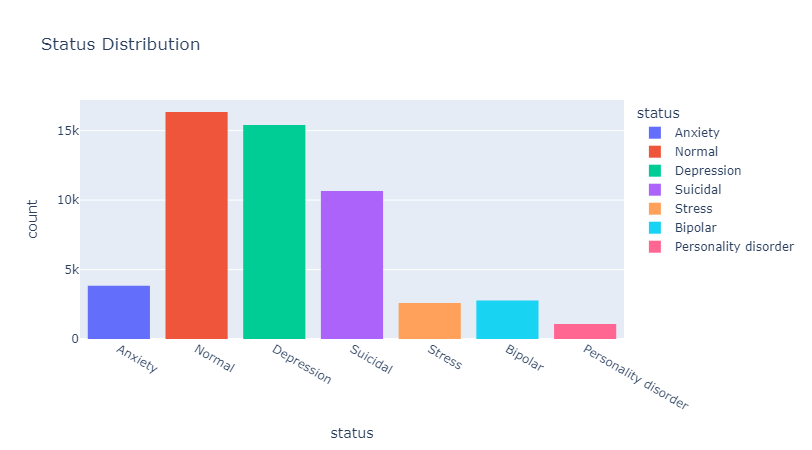
\includegraphics[width=0.75\textwidth]{images/class_distribution.png}
    \caption{Verteilung der mentalen Zustände im Datensatz}
    \label{fig:classdist}
\end{figure}

Die starke Dominanz der Kategorien \texttt{Normal}, \texttt{Depression} und \texttt{Suicidal} legt ein Klassenungleichgewicht nahe (z.\,B. Upsampling, Gewichtung bei Modellierung).


\subsection{Input– und Outputvariablen}
\begin{itemize}
    \item \textbf{Input}: Der bereinigte Fließtext aus der Spalte \texttt{statement}.
    \item \textbf{Output}: Die zugehörige Klassenvariable \texttt{label}, nominal skaliert.
\end{itemize}

\subsection{Prediction vs. Inference}
Die Zielsetzung dieses Projekts ist klar prognostischer Natur: Das Modell soll anhand unbekannter Social–Media–Texte automatisch den zugrundeliegenden mentalen Zustand erkennen. Dennoch sind auch inferenzielle Erkenntnisse möglich, z.\,B. welche Begriffe häufig in bestimmten Klassen auftreten oder welche Merkmale besonders trennscharf sind.

\subsection{Classification vs. Regression}
Die Klassifikation ist ein \textit{multinomiales Klassifikationsproblem}, da mehr als zwei Klassen vorhergesagt werden müssen.

\subsection{Korpusstruktur: N–Gramme}
Der aufbereitete Textkorpus umfasst insgesamt 5.961.315 Wortinstanzen (\textit{word tokens}) sowie 154.767 unterschiedliche Worttypen (\textit{word types}). Diese Kennzahlen geben Aufschluss über die Größe und Vielfalt des verwendeten Vokabulars.

\begin{figure}[h]
    \centering
    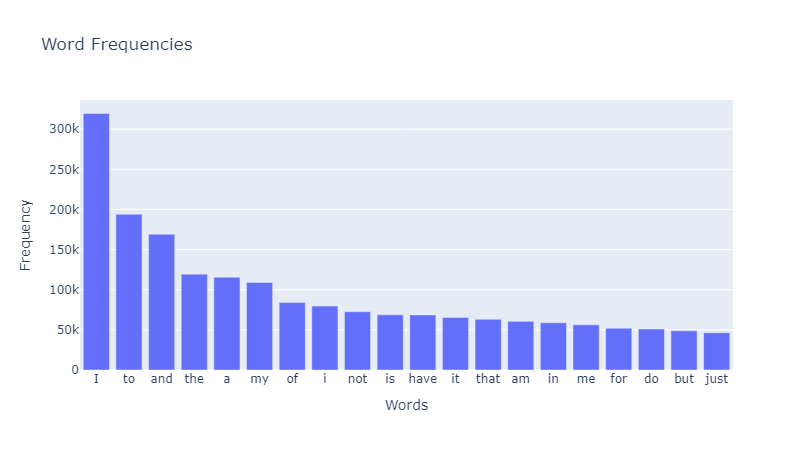
\includegraphics[width=0.75\textwidth]{images/word_frequencies.png}
    \caption{Häufigkeitsverteilung im Datensatz}
    \label{fig:wordfreq}
\end{figure}

Zur Beschreibung sprachlicher Muster wurden neben Unigrammen auch Bigramme betrachtet. Die häufigsten Bigramme (z.\,B. \textit{mental health}, \textit{feel like}) liefern semantische Hinweise auf häufig thematisierte Probleme.

\begin{figure}[h]
    \centering
    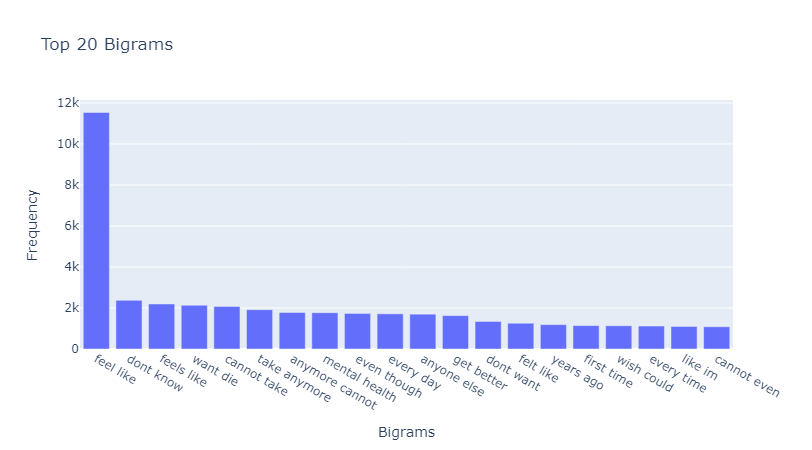
\includegraphics[width=0.75\textwidth]{images/bigrams.png}
    \caption{Verteilung der häufigsten Bigramme im Datensatz}
    \label{fig:bigrams}
\end{figure}

\subsection{Auffälligkeiten im Datensatz}

Bereits in der Phase des Data Understanding zeigten sich einige Auffälligkeiten:
\begin{itemize}
    \item Viele Texte enthalten HTML–
    
    Artefakte oder Sonderzeichen.
    \item Emojis, URLs und andere Rauschelemente stören die semantische Analyse.
    \item Die Labelverteilung ist stark unbalanciert,
    
    was die Modellgüte beeinträchtigen kann.
\end{itemize}
Diese Erkenntnisse flossen in die nachfolgende Vorverarbeitung ein.

\newpage

\subsection{Textvorverarbeitung}
Die manuelle Vorverarbeitung der Social-Media-Posts erfolgte in mehreren Stufen:

\begin{enumerate}
    \item \textbf{Kleinschreibung:}
    
    Im ersten Schritt der Textvorverarbeitung wurden alle Zeichen der Textvariable in Kleinbuchstaben umgewandelt, um die Konsistenz der Token zu gewährleisten und Redundanzen durch unterschiedliche Groß- und Kleinschreibung zu vermeiden:

\begin{lstlisting}[language=Python, caption={Umwandlung in Kleinschreibung}]
df["statement"] = df["statement"].str.lower()
\end{lstlisting}

    \item \textbf{Regex-Cleaning:}
    
    Zur Bereinigung wurden reguläre Ausdrücke eingesetzt.
    
    Die folgenden Python-Befehle illustrieren den Ablauf und sind Beispiele aus dem Code. Für eine vollständige Liste der verwendeten Regex-Befehle siehe das Jupyter-Notebook im Anhang.

\begin{lstlisting}[language=Python, caption={Regex-Cleaning der Social-Media-Texte}]

# Entfernen von URLs
df["statement"] = df["statement"].str.replace(r"https?://\S+|www\.\S+", "", regex=True)

# Entfernen von mentions
df["statement"] = df["statement"].str.replace(r"@\w+", "", regex=True)

# Entfernen von HTML-Entities und Zero-Width Characters (z.B., "&#x27;", "\u200b")
df["statement"] = df["statement"].str.replace(r'&#x[0-9a-fA-F]+;|\u200b', '', regex=True)
\end{lstlisting}

    \item \textbf{Stopword-Entfernung:}

Zur Reduktion nicht-informativer Wörter wurden sogenannte \textit{Stopwords} entfernt. Hierzu wurde die englische Stopword-Liste aus der Bibliothek \texttt{nltk} verwendet. Jedes Token wurde überprüft und bei Übereinstimmung mit einem Eintrag der Stopword-Liste entfernt:

\begin{lstlisting}[language=Python, caption={Entfernung englischer Stopwords mit nltk}]
import nltk
from nltk.corpus import stopwords

nltk.download('stopwords')
stop_words = set(stopwords.words('english'))

def remove_stopwords(text):
    return ' '.join([word for word in text.split() if word.lower() not in stop_words])

df["statement"] = df["statement"].apply(remove_stopwords)
\end{lstlisting}

Nach Abschluss der Vorverarbeitung wurde der Korpus deutlich reduziert:

Er umfasst nun 2.717.728 Wortvorkommen (\textit{word instances}) und 76.395 unterschiedliche Wortarten (\textit{word types}).

Diese Reduktion verdeutlicht den Effekt der Reinigungs- und Filterprozesse auf die sprachliche Komplexität des Datensatzes. Obwohl der bereinigte Korpus nun ausschließlich relevante Terme enthält, bleibt die Anzahl der Worttypen hoch. Daher wird im nächsten Schritt eine weiterführende Tokenisierung eingesetzt, um die lexikalische Vielfalt weiter zu verringern.

\begin{figure}[h]
    \centering
    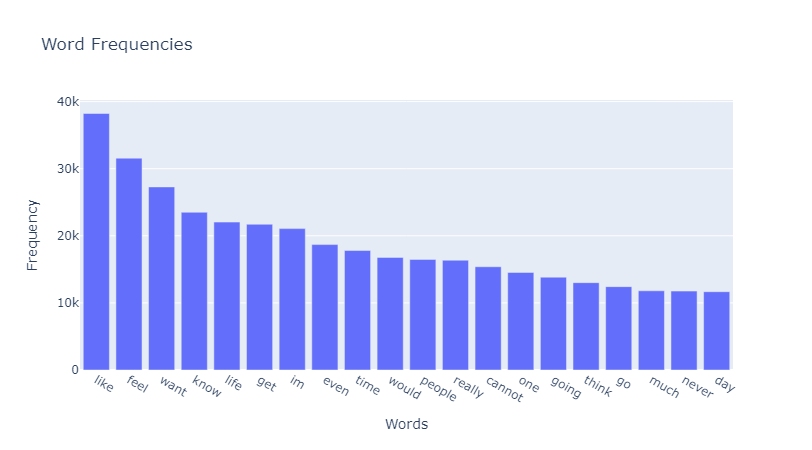
\includegraphics[width=0.75\textwidth]{images/new_word_frequencies.png}
    \caption{Verteilung der Wortinstanzen und -typen nach Bereinigung}
    \label{fig:newwordfreq}
\end{figure}

    \item \textbf{Tokenisierung:}
    
Zerlegung der bereinigten Texte in einzelne Token durch Leerzeichentrennung 

mittels \verb|.split()| oder mit regulären Ausdrücken:

\begin{lstlisting}[language=Python, caption={Tokenisierung mittels Regex}]
    tokens = re.findall(r"\w+", text)
\end{lstlisting}

    \item \textbf{weitere Visualisierung:}
    
    Zur explorativen Analyse des Korpus wurde eine Wordcloud erstellt, welche die häufigsten Begriffe aus der \texttt{statement}-Spalte visuell hervorhebt. Dabei werden besonders häufig vorkommende Wörter größer dargestellt, während seltenere Begriffe kleiner erscheinen. Diese Form der Visualisierung erlaubt einen schnellen Überblick über zentrale Themen und sprachliche Muster im Datensatz. Zusätzlich wurden Wordclouds für verschiedene \texttt{status}-Kategorien generiert, um potenzielle Unterschiede in der Wortwahl zwischen den Klassen zu erkennen.

\begin{figure}[h]
\centering
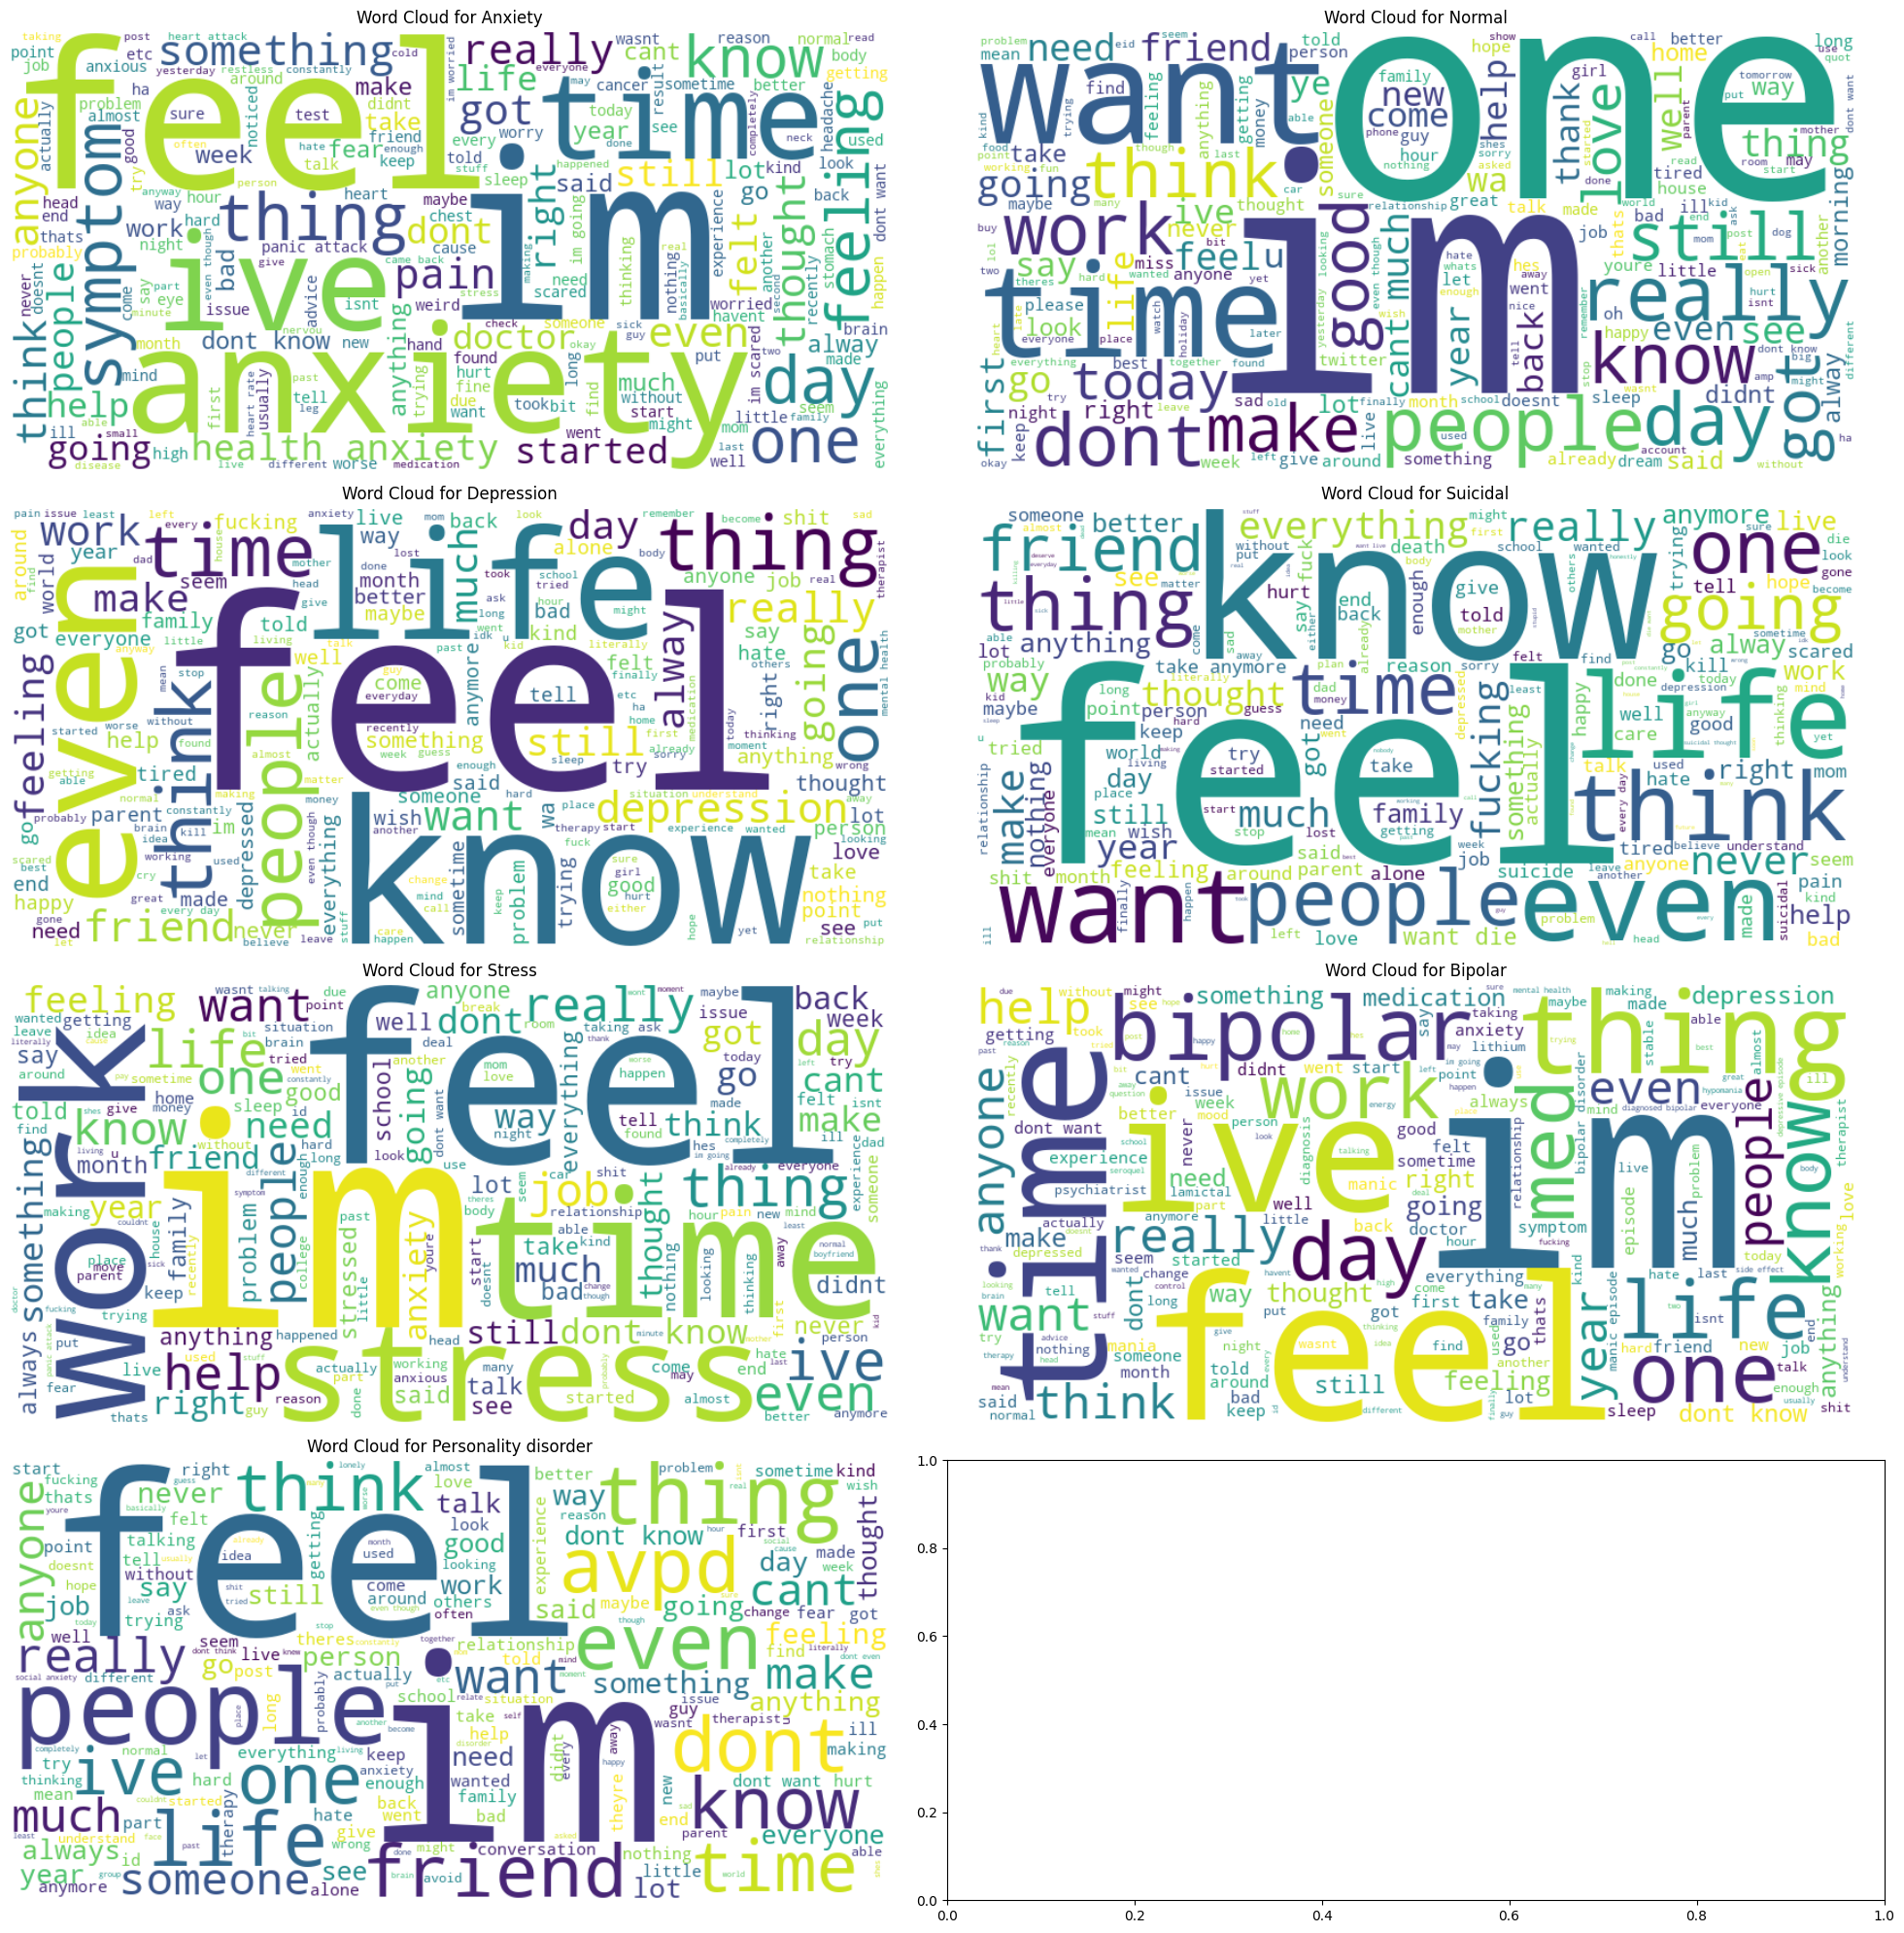
\includegraphics[width=0.75\textwidth]{images/wordcloud.png}
\caption{Wordclouds für verschiedene \texttt{status}-Kategorien}
\label{fig:wordcloud}
\end{figure}

\end{enumerate}

\newpage

\subsection{Feature-Engineering: Bag-of-Words und N-Gramme}

Im Rahmen des Feature-Engineering-Prozesses haben wir das 

Bag-of-Words-Verfahren verwendet, um die Textdaten in numerische Repräsentationen umzuwandeln, die von Maschinenmodellen verarbeitet werden können. 

Das Verfahren basiert auf der Idee, dass Text als eine Sammlung von Wörtern betrachtet wird, ohne dabei auf die grammatikalische Struktur oder die Reihenfolge der Wörter Rücksicht zu nehmen. Dies ermöglicht es uns, die Häufigkeit von Wörtern in einem Text als Merkmale zu extrahieren, was für viele maschinelle Lernaufgaben nützlich ist.

Wir haben den \texttt{CountVectorizer} 

aus der \texttt{scikit-learn}-Bibliothek 

genutzt, um eine Merkmalsmatrix zu erstellen. 

Der \texttt{CountVectorizer} analysiert das Korpus und zählt, wie oft jedes Wort in den Dokumenten vorkommt. 

Durch die Auswahl von Monogrammen, also einzelne Wörter und Bigrammen, also Paare aufeinanderfolgender Wörter, wurde berücksichtigt, dass nicht nur einzelne Wörter, sondern auch Kombinationen von benachbarten Wörtern (wie z.\,B. mental health) wichtige Kontextinformationen für die Modellvorhersage liefern können.

Dies ermöglicht es, einfache semantische Beziehungen zwischen den Wörtern zu erfassen.

Um sicherzustellen, dass das Modell nicht nur auf den Trainingsdaten, 

sondern auch auf neuen, unsichtbaren Daten gut funktioniert, haben wir die Daten in

Trainings- und Testdatensätze aufgeteilt.

Dies geschah durch eine zweifache Anwendung von \verb|train_test_split|, um sowohl eine Modell als auch eine Validierungsaufteilung zu erzeugen. 

Der \verb|CountVectorizer| wurde dann auf den Trainingsdatensatz angewendet, um die Merkmale zu extrahieren und auf den Testdatensatz transformiert, um sicherzustellen, dass das Modell auf neuen Daten generalisieren kann.

Zusätzlich wurde die maximale Anzahl an Features auf 5000 begrenzt, um die Anzahl der Merkmale zu reduzieren und eine Überanpassung des Modells zu verhindern, was die Effizienz des Trainingsprozesses verbessert.